\documentclass[11pt,a4paper]{article}
\usepackage{graphicx}
\usepackage{isabelle,isabellesym}
\usepackage{amssymb}
\usepackage{wasysym}
\usepackage[utf8]{inputenc}
\usepackage[only,bigsqcap]{stmaryrd}
%\usepackage{masmath}

% this should be the last package used
\usepackage{pdfsetup}

\newcommand{\isasymNoMsg}{\ensuremath\varepsilon}
%\newcommand{\isasymMsg}{\texttt{Msg}}
%\newcommand{\isasymMsg}{\isatext{\rm\sffamily{}Msg}}
\newcommand{\isasymMsg}{\textsf{Msg}}
% \newcommand{\isasymB}{\textsf{B}}
% \newcommand{\isasymR}{\textsf{R}}
% \newcommand{\isasymS}{\textsf{S}}
% \newcommand{\isasymU}{\textsf{U}}
% \newcommand{\isasymW}{\textsf{W}}

\newcommand{\backslashlessgreater}[1]{\ensuremath{\backslash\!\!<}#1\ensuremath{>}}
\newcommand{\isasymHTMLNoMsg}{\backslashlessgreater{HTMLNoMsg}}
\newcommand{\isasymHTMLMsg}{\backslashlessgreater{HTMLMsg}}



\urlstyle{rm}
\isabellestyle{it}
\pagestyle{myheadings}

\begin{document}

\title{AutoFocus Stream Processing for Single-Clocking and Multi-Clocking Semantics}
\author{David Trachtenherz}
\maketitle

\begin{abstract}
We formalize the AutoFocus Semantics (a time-synchronous subset of the
Focus formalism) as stream processing functions on finite and infinite
message streams represented as finite/infinite lists. The
formalization comprises both the conventional single-clocking
semantics (uniform global clock for all components and communications
channels) and its extension to multi-clocking semantics (internal
execution clocking of a component may be a multiple of the external
communication clocking). The semantics is defined by generic stream
processing functions making it suitable for simulation/code generation
in Isabelle/HOL. Furthermore, a number of AutoFocus semantics
properties are formalized using definitions from the Nat-Interval-Logic
theories.
\end{abstract}

\tableofcontents

\begin{center}
  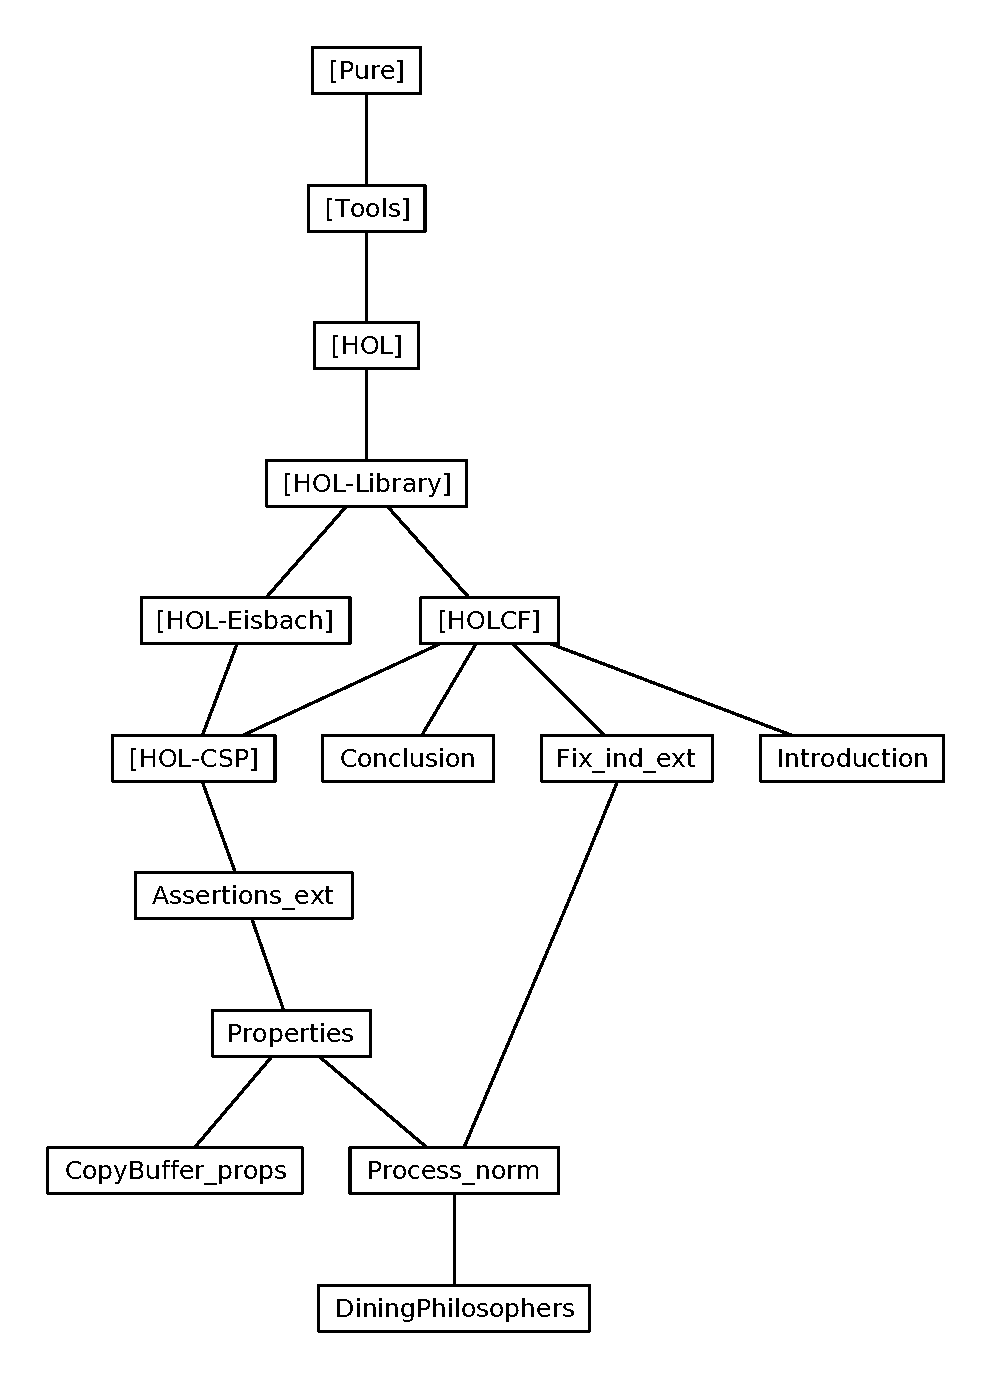
\includegraphics[scale=0.5]{session_graph}
\end{center}

\clearpage

\parindent 0pt\parskip 0.5ex
\input{session}

\end{document}
